\section{Authentication using OpenPGP\index{OpenPGP keys} keys}
This authentication method is part of the certificate authentication
method in \gnutls{}. All the key exchange methods shown in \hyperref{figure}{figure }{}{fig:cert} are
available in OpenPGP authentication. 

\subsection{The OpenPGP trust model in \gnutls{}}
\label{sec:pgp}

\subsubsection{The OpenPGP trust model}

The OpenPGP key authentication relies on a distributed trust model, called
the "web of trust". The "web of trust" uses a decentralized system of 
trusted introducers, which are the same as a CA. OpenPGP allows anyone to 
sign anyone's else public key. When Alice signs Bob's key, she is introducing 
Bob's key to anyone who trusts Alice. If someone trusts Alice to introduce
keys, then Alice is a trusted introducer in the mind of that observer.

\begin{figure}[hbtp]
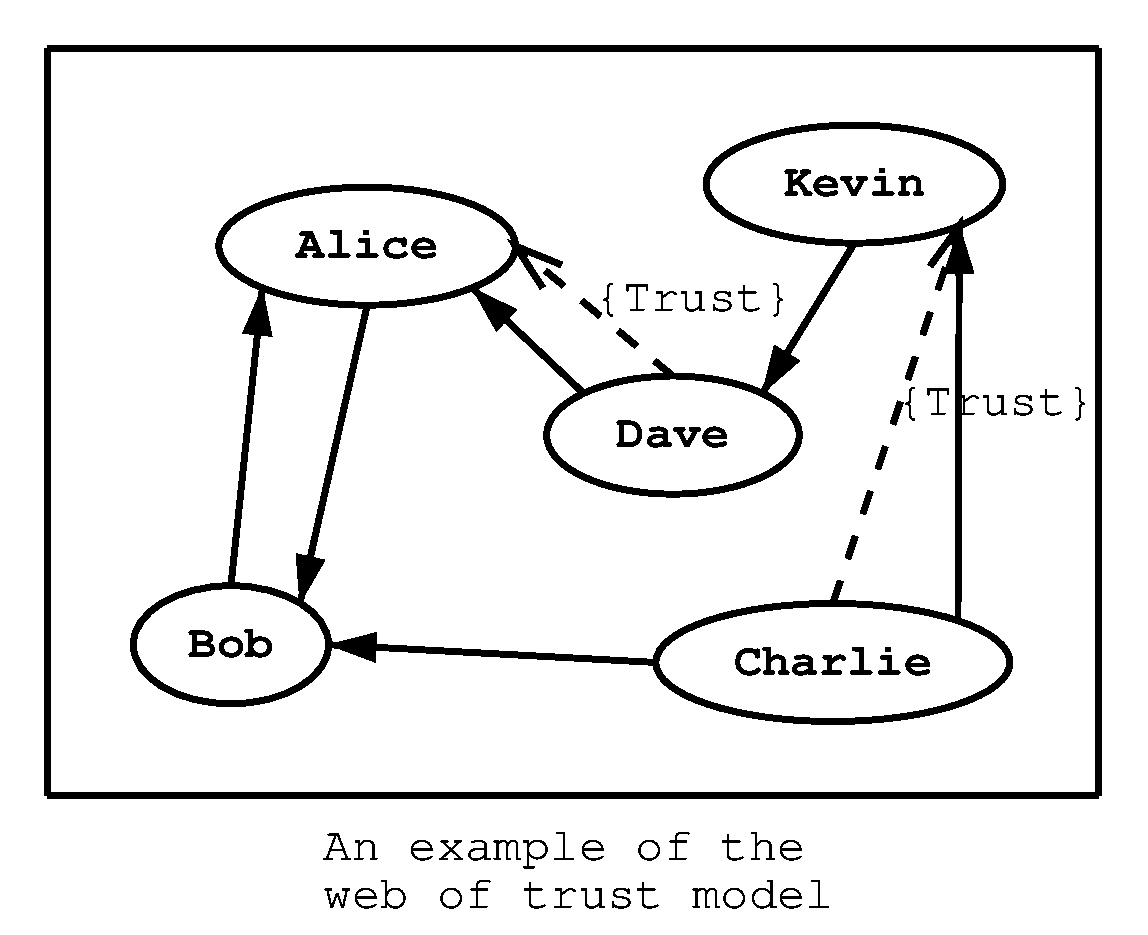
\includegraphics[height=9cm,width=11cm]{pgp-fig1}
\label{fig:pgp1}
\end{figure}

For example: If David trusts Alice to be an introducer, and Alice signed
Bob's key, Dave also trusts Bob's key to be the real one.

There are some key points that are important in that model. In the example
Alice has to sign Bob's key, only if she is sure that the key belongs
to Bob. Otherwise she may also make Dave falsely believe that this
is Bob's key. Dave has also the responsibility to know who to trust.
This model is similar to real life relations.

Just see how Charlie behaves in the previous example. Although he has 
signed Bob's key - because he knows, somehow, that it belongs to Bob - 
he does not trust Bob to be an introducer. Charlie decided to trust only 
Kevin, for some reason. A reason could be that Bob is lazy enough, and 
signs other people's keys without being sure that they belong to the 
actual owner.


\subsubsection{GnuTLS functions}

First we've to differentiate between ownertrust and validity. Sometimes trust
and validity is used as a synonym but this is not correct.
\par
The ownertrust describes how trustworthy the signature of a special
key owner is. Even if we've three or more signatures to make a key valid,
it's possible that we don't trust the owner at all and thus we don't trust 
the signature he made. There are different ownertrust levels:
\begin{enumerate}
\item Don't know
\item I do NOT trust
\item I trust marginally
\item I trust fully
\item I trust ulitmately.
\end{enumerate}

For example we need three marginally trusted signature to make a key
valid or one full trusted signature. The ultimate trust is only used
when we are the owner of a key and we also have the secret key.
\par
In the case we don't trust the owner, those signatures are skipped
for the web of trust calculation.
\par
All checks in GnuTLS are done in \printfunc{gnutls_openpgp_verify_key}{gnutls\_openpgp\_verify\_key}. 
If a trustdb is available, this is the file which contains all information about the
key owner (ownertrust), additional checks are performed.
\\
First we get the trustdb entry to see if the key is not disabled because
those keys shouldn't be used at all. Another possible case is that we
don't trust the key, which means we don't need to perform further checks.
\par
If the ownertrust is at least marginal we continue to check all signatures
the key contains to get the validity of the key. It is likely that the
public keyring does not contain all needed keys to check all signatures.
When a signature could not be checked due to a missing key, the function 
tries the next signature. When NO public key is available, the function
checks at least the self signature which must be valid in any case because
it was created by the key itself.
\\
Validity means if the signatures on the key are valid and the key was not 
changed by somebody or corrupted during transport.


